\documentclass[border=3pt,tikz]{standalone}
\usepackage{amsmath}

\usetikzlibrary {3d} 
\usetikzlibrary {arrows}
\usetikzlibrary{shapes.geometric}
\begin{document}
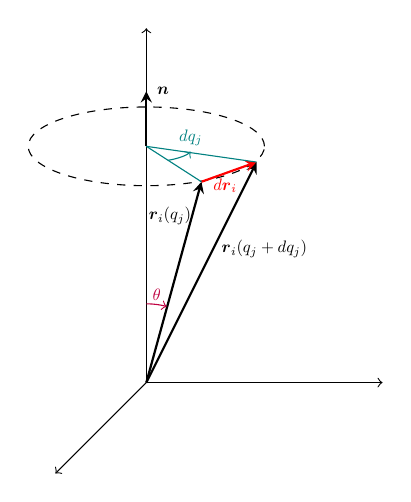
\begin{tikzpicture} %[=>stealth]
    \tikzset{
        partial ellipse/.style args={#1:#2:#3}{
            insert path={+ (#1:#3) arc (#1:#2:#3)}
        }
    }
      \draw [->] (0,0) -- (xyz cs:x=3);
      \draw [->] (0,0) -- (xyz cs:y=4.5);
      \draw [->] (0,0) -- (xyz cs:z=3); 
      \draw [dashed] (0.0,3.0) ellipse (1.5 and 0.5);
      \draw [thick, -{stealth}] (0, 0) -- (xyz cs:x=0.7,y=2.55);
      \node[below, scale=.6] at (0.3, 2.3) {$\boldsymbol{r}_i (q_j)$};
      \draw [thick, -{stealth}] (0, 0) --(xyz cs:x=1.4,y=2.8);
      \node[scale=.6] at (1.5, 1.7) {$\boldsymbol{r}_i (q_j+dq_j)$};
      \draw [red, thick, -{stealth}] (0.7, 2.55) -- (1.4, 2.8);
      \node[red, scale=.6] at (1.0, 2.5) {$d\boldsymbol{r}_i$};
      \draw [thick, -{stealth}] (0, 3) -- (0, 3.7) node[right, scale=0.6] {$\;\boldsymbol{n}$};
    
      \draw [teal] (0, 3) -- (0.7, 2.55);
      \draw [teal] (0, 3) -- (1.4, 2.8);
      \draw[teal, ->] (0, 3.0) [partial ellipse=297:340:0.6 and 0.2] node[above, scale=0.6] {$dq_j$} ;
      \draw[purple, ->] (0, 0) [partial ellipse=90:75:1 and 1] node[above left, scale=0.6] {$\theta$} ;
    \end{tikzpicture}
\end{document}